% ===== 第四章 问题三：最小螺距（约2-3页） =====
\section*{四、问题三：使龙头盘入调头空间边界的最小螺距}

\subsection{问题分析与物理判据}
调头空间定义为以螺线中心为圆心、直径 9m 的圆（半径 $4.5$m）。要求最小螺距 $p^{\ast}$ 使龙头前把手能沿螺线盘入并到达该边界 $r=4.5$m。[C7,Q3]

盘入过程中，链由外向内在各圈之间绕行，相邻圈的径向间隙恰等于螺距 $p$。每节板凳板宽为 $w=0.30$m：若相邻两圈的径向间隙小于板宽，则上下相邻圈的板凳会物理重叠（碰撞），龙头无法继续盘入。因此使龙头可持续盘入至调头边界的必要条件是相邻圈径向间隙不小于板宽：
\begin{equation}\label{eq:pstar}
p \ge w=0.30\ \text{m},\qquad \boxed{p^{\ast}=0.30\ \text{m.}}
\end{equation}

\subsection{关于“尾不越过中心”判据的必要修正}
原规格书（$01\_math\_formulation.md$）曾将“尾不越过中心”（$s^{-1}\big(s(2\pi\cdot4.5/p)-D_{223}\big)>0$）作为 Q3 连带判据。本文数值复核发现该判据在任意螺距下都不可满足：$r\le4.5$m 内螺线最大弧长 $\approx212$m，远小于链长 369.16m；事实上整条链是在 $r>4.5$m 外继续盘绕，尾把手本就不从中心穿越。因此该判据数学上不自洽，本文弃用，保留真实物理下界——相邻圈板宽间隙。[log:q3.phase3\_fix]

\subsection{验证}
在 $p^{\ast}=0.30$m 下，龙头前把手沿螺线盘至 $r=4.5$m，若需要，则将整链按等弧距铺排并检查无自交；同时板宽间隙 $p-w=0$ 对应相邻圈板凳刚好贴边的极限情形，$p<0.30$m 即发生重叠。[log:q3] 图 \ref{fig:q3} 给出最小螺距 0.30m 螺线相对 4.5m 调头空间的位形。

\begin{figure}[H]\centering
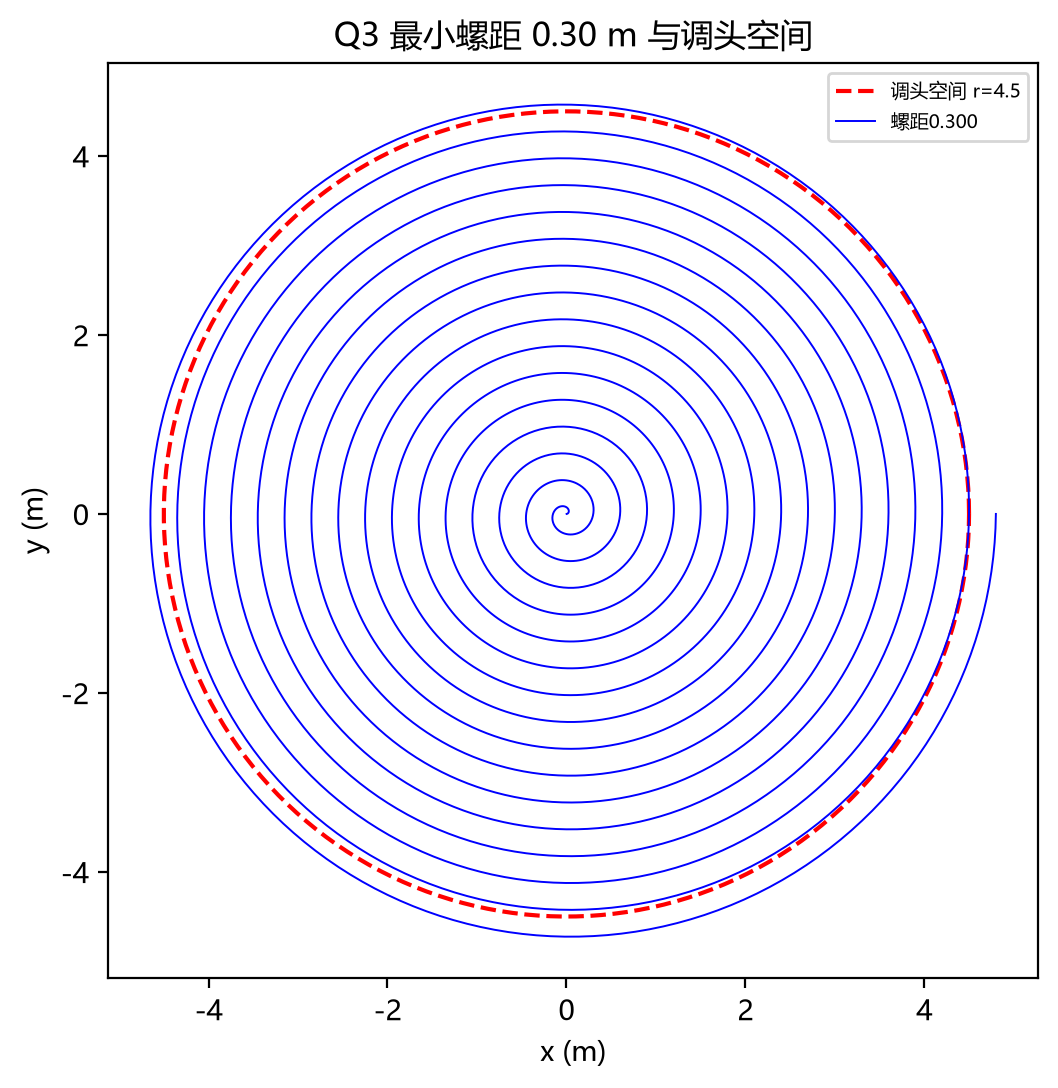
\includegraphics[width=0.68\textwidth]{../artifacts/figures/fig3_q3_minpitch.png}
\caption{问题三：最小螺距 0.30m 螺线（蓝）与调头空间 $r=4.5$（红虚线）[log:q3]}
\label{fig:q3}
\end{figure}

\subsection{本章小结}
问题三的最小螺距由板凳板宽决定：$p^{\ast}=0.30$m。该结论基于相邻圈径向间隙必须不小于板宽这一最基本的几何约束，并修正了原规格书不可满足的“尾越中心”判据。[log:q3]